\section{Import \& Export}

\begin{figure}
  \centering
  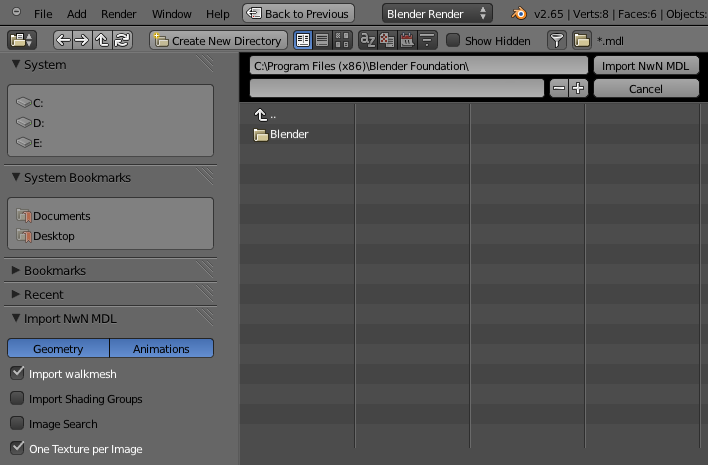
\includegraphics[trim=0 0 0 0, clip, width=\textwidth]{import01}
  \caption[mdl import]{Import Screen}
  \label{fig:import01}
\end{figure}

\begin{description}
    \item[Geometry \& Animation] Either import the geometry, animations or both. Note that the animations may not work, if the animated objects are not present. However you may add the animations to other objects manually.
    \item[Import Walkmesh] Attempts to import a walkmesh. If the imported model is a placeable, the script will look for a {\textit{*.pwk}} file in the same folder. If the model is a door, it will look for a {\textit{*.dwk}} file. If the model is a tile, it will read the walkmesh directly from the {\textit{*.mdl}} file.
    \item[Import Shading Groups] Import shading groups for faces. Shading groups are not supported by Blender, i.e. it will have no effect on the displayed model in blender. An imported shading group is converted to a vertex group, containing all vertices of the faces belonging the shading group.
    \item[Image Search] Enable this to search for textures in subdirectories. (This may be slow)
    \item[One Texture per Image] When this is enabled, the import script will create only one texture for every image found in the model file. When disabled, every node will get it's own texture, even if it's image has already been loaded to a different texture previously.
\end{description}
